% This file was created with tikzplotlib v0.10.1.
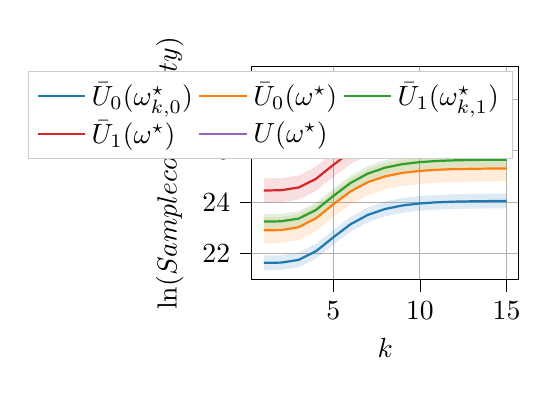
\begin{tikzpicture}

\definecolor{crimson2143940}{RGB}{214,39,40}
\definecolor{darkgray176}{RGB}{176,176,176}
\definecolor{darkorange25512714}{RGB}{255,127,14}
\definecolor{forestgreen4416044}{RGB}{44,160,44}
\definecolor{lightgray204}{RGB}{204,204,204}
\definecolor{mediumpurple148103189}{RGB}{148,103,189}
\definecolor{steelblue31119180}{RGB}{31,119,180}

\begin{axis}[
legend cell align={left},
legend columns=3,
legend style={fill opacity=1, draw opacity=1, text opacity=1, draw=lightgray204},
tick align=outside,
tick pos=left,
width=0.41\columnwidth,
x grid style={darkgray176},
xlabel={\(\displaystyle k\)},
xmajorgrids,
xmin=0.3, xmax=15.7,
xtick style={color=black},
y grid style={darkgray176},
ylabel={\(\displaystyle \ln(Sample complexity)\)},
ymajorgrids,
ymin=20.9725325868307, ymax=29.2757663372702,
ytick style={color=black}
]
\path [fill=steelblue31119180, fill opacity=0.15]
(axis cs:1,21.9226235307899)
--(axis cs:1,21.3499523027598)
--(axis cs:2,21.3601240666647)
--(axis cs:3,21.4651943640181)
--(axis cs:4,21.7991339815673)
--(axis cs:5,22.3396650912369)
--(axis cs:6,22.8523010836422)
--(axis cs:7,23.2185322806461)
--(axis cs:8,23.4494833755461)
--(axis cs:9,23.5867791809039)
--(axis cs:10,23.6657767186607)
--(axis cs:11,23.7103072764993)
--(axis cs:12,23.7349826302463)
--(axis cs:13,23.748581366947)
--(axis cs:14,23.7559456792944)
--(axis cs:15,23.7599556312462)
--(axis cs:15,24.3328655481706)
--(axis cs:15,24.3328655481706)
--(axis cs:14,24.3288514322916)
--(axis cs:13,24.321492146963)
--(axis cs:12,24.307903654503)
--(axis cs:11,24.2832476484922)
--(axis cs:10,24.2387535030656)
--(axis cs:9,24.159838516731)
--(axis cs:8,24.0227194594934)
--(axis cs:7,23.7921545882558)
--(axis cs:6,23.4266775978881)
--(axis cs:5,22.9148220255386)
--(axis cs:4,22.3736801325304)
--(axis cs:3,22.0383218520977)
--(axis cs:2,21.9328679069213)
--(axis cs:1,21.9226235307899)
--cycle;

\path [fill=darkorange25512714, fill opacity=0.15]
(axis cs:1,23.408487145154)
--(axis cs:1,22.4004722915767)
--(axis cs:2,22.4105728034589)
--(axis cs:3,22.5220836624547)
--(axis cs:4,22.866531011331)
--(axis cs:5,23.4099654580382)
--(axis cs:6,23.9175288406959)
--(axis cs:7,24.2780605397594)
--(axis cs:8,24.5051044422648)
--(axis cs:9,24.6399874100174)
--(axis cs:10,24.7175372630883)
--(axis cs:11,24.761203005187)
--(axis cs:12,24.7854351250804)
--(axis cs:13,24.7987358740842)
--(axis cs:14,24.8059742217163)
--(axis cs:15,24.8098860821196)
--(axis cs:15,25.8181805157961)
--(axis cs:15,25.8181805157961)
--(axis cs:14,25.8142596469336)
--(axis cs:13,25.8070051921959)
--(axis cs:12,25.7936761792341)
--(axis cs:11,25.7693957491165)
--(axis cs:10,25.7256505713103)
--(axis cs:9,25.6479780065235)
--(axis cs:8,25.5129310593682)
--(axis cs:7,25.2857135376155)
--(axis cs:6,24.9251135395744)
--(axis cs:5,24.4177007957772)
--(axis cs:4,23.8743739897777)
--(axis cs:3,23.5300714541727)
--(axis cs:2,23.4187749386286)
--(axis cs:1,23.408487145154)
--cycle;

\path [fill=forestgreen4416044, fill opacity=0.15]
(axis cs:1,23.5308330767636)
--(axis cs:1,22.9587434871178)
--(axis cs:2,22.9689977863516)
--(axis cs:3,23.0740400323195)
--(axis cs:4,23.4080637815444)
--(axis cs:5,23.9488755507292)
--(axis cs:6,24.4619275823764)
--(axis cs:7,24.8284112714021)
--(axis cs:8,25.0594780140553)
--(axis cs:9,25.1968427393678)
--(axis cs:10,25.2758676839574)
--(axis cs:11,25.3203895390778)
--(axis cs:12,25.3451105058861)
--(axis cs:13,25.3586861807414)
--(axis cs:14,25.3660750666784)
--(axis cs:15,25.3700693698522)
--(axis cs:15,25.9423223697926)
--(axis cs:15,25.9423223697926)
--(axis cs:14,25.9383322530162)
--(axis cs:13,25.9309474329301)
--(axis cs:12,25.9173807310938)
--(axis cs:11,25.8926768178183)
--(axis cs:10,25.8481929386623)
--(axis cs:9,25.7692511571519)
--(axis cs:8,25.6320648874253)
--(axis cs:7,25.4013915639822)
--(axis cs:6,25.0356583185963)
--(axis cs:5,24.5234102454968)
--(axis cs:4,23.9820145288074)
--(axis cs:3,23.6465659402843)
--(axis cs:2,23.5411475529112)
--(axis cs:1,23.5308330767636)
--cycle;

\path [fill=crimson2143940, fill opacity=0.15]
(axis cs:1,24.9266711658687)
--(axis cs:1,23.983751873894)
--(axis cs:2,23.9946085510208)
--(axis cs:3,24.100313568715)
--(axis cs:4,24.4352098845044)
--(axis cs:5,24.9762304969795)
--(axis cs:6,25.4888190044475)
--(axis cs:7,25.8550200524069)
--(axis cs:8,26.0860350540486)
--(axis cs:9,26.2234165592968)
--(axis cs:10,26.3024768768282)
--(axis cs:11,26.3470273099851)
--(axis cs:12,26.3717641112726)
--(axis cs:13,26.3853483669089)
--(axis cs:14,26.3927437821274)
--(axis cs:15,26.3967417668942)
--(axis cs:15,27.3397295276526)
--(axis cs:15,27.3397295276526)
--(axis cs:14,27.3357384290508)
--(axis cs:13,27.3283558098935)
--(axis cs:12,27.3147952926842)
--(axis cs:11,27.2901024483692)
--(axis cs:10,27.2456334741359)
--(axis cs:9,27.1667245621961)
--(axis cs:8,27.029625957477)
--(axis cs:7,26.7991256134965)
--(axis cs:6,26.4337741872402)
--(axis cs:5,25.9220045961541)
--(axis cs:4,25.3803966492865)
--(axis cs:3,25.0439755350714)
--(axis cs:2,24.9376407119502)
--(axis cs:1,24.9266711658687)
--cycle;

\path [fill=mediumpurple148103189, fill opacity=0.15]
(axis cs:1,28.8983466213412)
--(axis cs:1,27.7482875698782)
--(axis cs:2,27.7482875698782)
--(axis cs:3,27.7482875698782)
--(axis cs:4,27.7482875698782)
--(axis cs:5,27.7482875698782)
--(axis cs:6,27.7482875698782)
--(axis cs:7,27.7482875698782)
--(axis cs:8,27.7482875698782)
--(axis cs:9,27.7482875698782)
--(axis cs:10,27.7482875698782)
--(axis cs:11,27.7482875698782)
--(axis cs:12,27.7482875698782)
--(axis cs:13,27.7482875698782)
--(axis cs:14,27.7482875698782)
--(axis cs:15,27.7482875698782)
--(axis cs:15,28.8983466213412)
--(axis cs:15,28.8983466213412)
--(axis cs:14,28.8983466213412)
--(axis cs:13,28.8983466213412)
--(axis cs:12,28.8983466213412)
--(axis cs:11,28.8983466213412)
--(axis cs:10,28.8983466213412)
--(axis cs:9,28.8983466213412)
--(axis cs:8,28.8983466213412)
--(axis cs:7,28.8983466213412)
--(axis cs:6,28.8983466213412)
--(axis cs:5,28.8983466213412)
--(axis cs:4,28.8983466213412)
--(axis cs:3,28.8983466213412)
--(axis cs:2,28.8983466213412)
--(axis cs:1,28.8983466213412)
--cycle;

\addplot [thick, steelblue31119180]
table {%
1 21.6362879167748
2 21.646495986793
3 21.7517581080579
4 22.0864070570489
5 22.6272435583877
6 23.1394893407651
7 23.505343434451
8 23.7361014175198
9 23.8733088488175
10 23.9522651108632
11 23.9967774624958
12 24.0214431423747
13 24.035036756955
14 24.042398555793
15 24.0464105897084
};
\addlegendentry{$\bar U_0(\omega_{k,0}^\star)$}
\addplot [thick, darkorange25512714]
table {%
1 22.9044797183653
2 22.9146738710437
3 23.0260775583137
4 23.3704525005544
5 23.9138331269077
6 24.4213211901351
7 24.7818870386874
8 25.0090177508165
9 25.1439827082705
10 25.2215939171993
11 25.2652993771518
12 25.2895556521573
13 25.3028705331401
14 25.310116934325
15 25.3140332989578
};
\addlegendentry{$\bar U_0(\omega^\star)$}
\addplot [thick, forestgreen4416044]
table {%
1 23.2447882819407
2 23.2550726696314
3 23.3603029863019
4 23.6950391551759
5 24.236142898113
6 24.7487929504863
7 25.1149014176922
8 25.3457714507403
9 25.4830469482598
10 25.5620303113099
11 25.606533178448
12 25.6312456184899
13 25.6448168068357
14 25.6522036598473
15 25.6561958698224
};
\addlegendentry{$\bar U_1(\omega_{k,1}^\star)$}
\addplot [thick, crimson2143940]
table {%
1 24.4552115198813
2 24.4661246314855
3 24.5721445518932
4 24.9078032668955
5 25.4491175465668
6 25.9612965958438
7 26.3270728329517
8 26.5578305057628
9 26.6950705607464
10 26.7740551754821
11 26.8185648791772
12 26.8432797019784
13 26.8568520884012
14 26.8642411055891
15 26.8682356472734
};
\addlegendentry{$\bar U_1(\omega^\star)$}
\addplot [thick, mediumpurple148103189]
table {%
1 28.3233170956097
2 28.3233170956097
3 28.3233170956097
4 28.3233170956097
5 28.3233170956097
6 28.3233170956097
7 28.3233170956097
8 28.3233170956097
9 28.3233170956097
10 28.3233170956097
11 28.3233170956097
12 28.3233170956097
13 28.3233170956097
14 28.3233170956097
15 28.3233170956097
};
\addlegendentry{$U(\omega^\star)$}
\end{axis}

\end{tikzpicture}
